\documentclass[11pt]{texMemo-gibbons}
\usepackage[english]{babel}
\usepackage{graphicx}
\usepackage{blindtext}
\usepackage{amsmath,amssymb,units}
\usepackage{siunitx}
\usepackage[outdir=./]{epstopdf}
\memostudent{Ty Davis}
\memocourse{ECE 3210}
\memosubject{Lab 5, LTI System Response to Periodic Signal}
\memodate{\today}
\logo{
\includegraphics[width=0.5\textwidth]{ece_horiz.pdf}}

\begin{document}
\maketitle

\section{Introduction}
\label{sec:introduction}

In this lab we are analyzing the LTI response of a system
to a periodic input. Similar to Lab 2 where we analyzed
the reponse of a system to a certain input, here the
input isn't a step or ramp, but rather a periodic input
where the system doesn't have complete time to settle
in between variations of the input.

The circuit that we are using is identical to the circuit in 
Lab 2, and is shown in Fig.~\ref{fig:circuit}. It is a simple
RLC circuit.


\section{Theory}
\label{sec:theory}

The circuit from Fig.~\ref{fig:circuit} is a simple
RLC circuit and the differential equation derived for
this circuit is shown in Eq.~\ref{eq:ode}.

\begin{equation}
  \Big(\text{D}^2 + \frac{1}{\text{R}\text{C}}\text{D} + \frac{1}{\text{L}\text{C}}\Big)y(t) = \Big(\frac{1}{\text{R}\text{C}}\text{D}\Big)f(t)
  \label{eq:ode}
\end{equation}

From this equation we can determine the system response $H(s)$,
shown in Eq.~\ref{eq:h(s)}

\begin{equation}
  H(s) = \frac{F(s)}{Y(s)} = \frac{\frac{1}{\text{R}\text{C}} s }{s^2 + \frac{1}{\text{R}\text{C}} s + \frac{1}{\text{L}\text{C}}}
  \label{eq:h(s)}
\end{equation}

This equation for the system response in the $s$ domain
is used to calculate $y(t)$. But first we need to find
the complex exponential Fourier Series representation
of the input. It follows the general form:

\begin{equation}
  f(t) \approx \sum_{n=-m}^{m}D_n e^{jn\omega_0 t}
  \label{eq:f(t)}
\end{equation}

Where the $D_n$ coefficients can be found using this equation:

\[
  D_n = \frac{1}{T_0} \int_{T_0}f_{T_0}(t) e^{-jn\omega_0 t} dt
\]

For this lab we are using a frequency of $f_0=20~\si{\kHz}$,
which leads to a period $T_0 = 0.05~\si{\ms}$ and fundamental
frequency $\omega_0 = 40000 \pi~\si{\Hz}$. 

Using these values, the expression for $D_n$ can be found in 
Eq.~\ref{eq:d_n}.

\begin{equation}
  D_n = \frac{80000}{n\omega_0} \big( 4 \sin (n \omega_0 T_0 / 4) \big)
  \label{eq:d_n}
\end{equation}

Now, all of these equations can be combined to find the system response $y(t)$
shown in Eq.~\ref{eq:y(t)}.

\begin{equation}
  y(t) = \sum _{-\infty}^{\infty} H(jn\omega_0) D_n e^{jn\omega_0 t}
  \label{eq:y(t)}
\end{equation}

\section{Results}
\label{sec:results}

Fig.~\ref{fig:plot} shows the analytical solution to
the system and the measured response. The two equations
that are shown in the analytical portion are from Eq.~\ref{eq:f(t)}
and Eq.~\ref{eq:y(t)}. Clearly, you can see that the
computed results line up very well with the measurements
that we found experimentally in the lab. It seems that the 
amplitide of the measurements is just slightly lower than
the computed solution, but that the values are remarkably
consistent.

\section{Discussion and Conclusions}
\label{sec:conclusions}

In this lab we managed to analyze the resopnse of an
LTI system to a periodic input. It seemed similar to
the analysis of the circuit from Lab 2, but we only
analyzed the impulse response of the circuit at that
time. The impulse response decayed slowly when compared
to the width of an impulse function. Naturally, as any
input function can be seen as the the impulse function
stacked alongside itself many times at varying amplitudes,
the response will then fall upon itself many times and
never find a chance to settle.



\clearpage

\begin{figure}[h!]
  \centering
  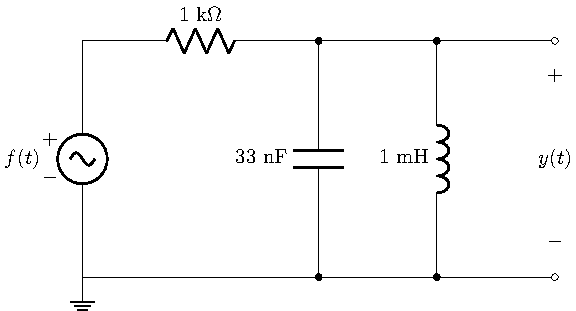
\includegraphics[width=0.7\linewidth]{circuits/circuit_01.pdf}
  \caption{The Circuit Used in the Lab}
  \label{fig:circuit}
\end{figure}

\begin{figure}[h!]
  \centering
  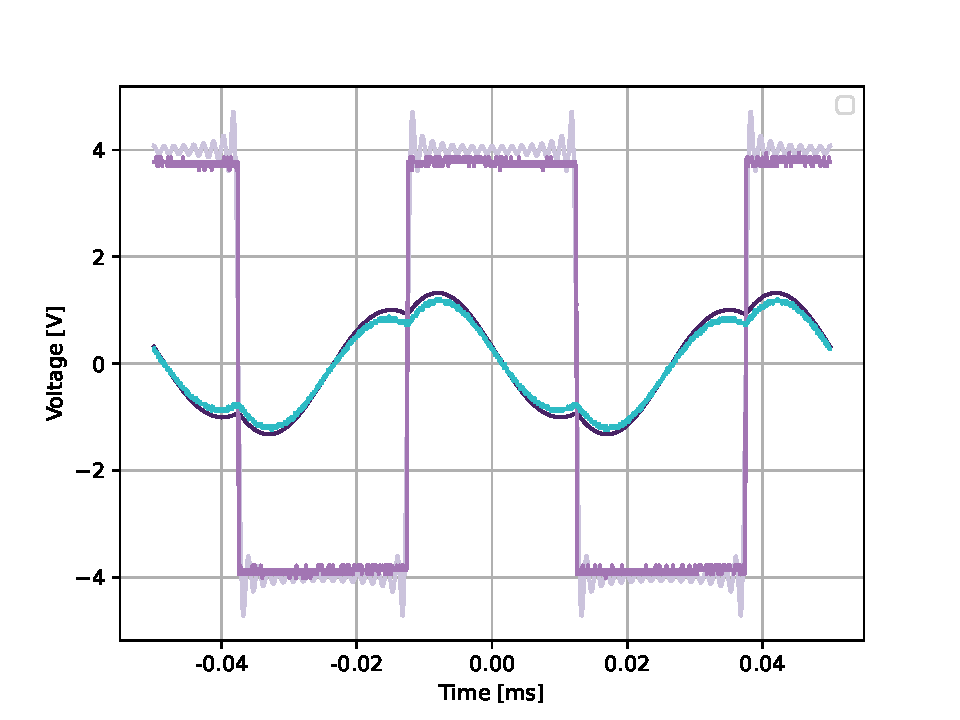
\includegraphics[width=0.7\linewidth]{plots/fourier_analysis.pdf}
  \caption{Analytical and Measured Results}
  \label{fig:plot}
\end{figure}



\end{document}
%%% Local Variables:
%%% mode: latex
%%% TeX-master: t
%%% End:
